\section{Theorie}
\label{sec:Theorie}
Gegenstand dieses Versuchs sind $\gamma$- und $\beta$-Strahlung und ihre Wechselwirkung mit Materie.
Ein Maß für die Warscheinlichkeit der Wechselwirkung zwischen Strahlung und Absorbermaterial ist der
Wirkungsqueerschnitt $\sigma$. Dieser steht in keinem Zusammenhang zur der geometrischen Größe, allerdings
ist die Anzahl der Wechselwirkungen abhängig von der Dicke des Absorbermaterials. Es ergibt sich ein
exponentieller Zusammenhang:
\begin{align}
N(D)=N_\mathrm{0}e^{-n\sigma D}.\label{eqn:abs}
\end{align}
Hier beschreibt $N_\mathrm{0}$ die Ausgangsaktivität, $D$ die Dicke und $n$ die Anzahl der Teilchen pro
Volumen im Absorber. Als Absorptionskoeffizient wird $n\cdot\sigma=\mu$ bezeichnet, diese Größe lässt sich
leicht messen und damit ergibt sich eine Abschätzung für den Wirkungsquerschnitt:
\begin{align}
\sigma=\frac{\mu}{n}=\frac{\mu M}{zN_\mathrm{A}\rho}.
\end{align}
$N_\mathrm{A}$ ist die Avogadro-Konstante, $\rho$ die Dichte, $M$ das Molekulargewicht und $z$ die Ordnungszahl.
Für $n$ gilt:
\begin{align}
\frac{zN_\mathrm{L}}{V_\mathrm{Mol}}.
\end{align}
Das molare Volumen wird als $V_\mathrm{Mol}$ bezeichnet.
\subsection{Gamma-Strahlung}
Atomkerne besitzen unterschiedliche Energieniveaus, fällt ein angeregter Kern in ein weniger angeregten Zustand, so
wird $\gamma$-Strahlung freigesetzt. $\gamma$-Strahlung besitz ein diskretes Energiespektrum.
Bei der Wechselwirkung mit Materie sind die wichtigsten Effekte der Photo-Effekt, der Compton-Effekt und
die Paarbildung.
Beim Photo-Effekt wird ein Elektron durch ein Photon aus dem Absorbermaterial rausgelöst. Da es zur Vernichtung des
Photons kommt, wird seine Energie vollständig an das Elektron abgegeben.
Beim Compton-Effekt gibt ein Photon nur einen Teil seiner Energie an ein Elektron ab und wird am Elektron gestreut.
Der Wirkungsqueerschnitt für diesen Vorgang ist definiert durch:
\begin{align}
\sigma_\mathrm{com}=2\pi r_\mathrm{e}^2\left(\frac{1+\varepsilon}{\varepsilon^2}\left[\frac{2(1+\varepsilon)}{1+2\varepsilon}-\frac{ln(1+2\varepsilon)}{\varepsilon}\right]+\frac{ln(1+2\varepsilon)}{2\varepsilon}-\frac{1+3\varepsilon}{(1+2\varepsilon)^2}\right)\label{eqn:sigma}.
\end{align}
$\varepsilon$ beschreibt das Verhältnis von Quantenenergie zur Ruheenergie des Elektrrons und $r_\mathrm{e}$
den klassischen Elektronenradius.
Die Paarbildung kommt nur zu Stande, wenn die Energie des $\gamma$-Quants mindestens doppelt so hoch ist wie
die Ruhemasse des Elektrons. Dabei wird das $\gamma$-Quant anihiliert und es entsteht ein Elektron und ein Positron.
Diese drei Effekte beeinflussen den Absorptionskoeffizienten $\mu$.
\subsection{Beta-Strahlung}
Besitzt ein Atomkern eine instabile Anordnung von Protonen und Elektronen, so werden diese in Form von $\beta$-Strahlung
emittiert, der Kern gejt in einen stabileren Zustand über. Ein Kernteilchen wird Umgewandelt nach:
\begin{align}
n \textrightarrow p+\beta^- +\overline{\nu_\mathrm{e}}\\
p \textrightarrow n+\beta^+ +\nu_\mathrm{e}.
\end{align}
Hierbei sind $p$ und $n$ Proton und Neutron, $\beta^-$ und $\beta^+$ Elektron und Positron und $\overline{\nu_\mathrm{e}}$ und $\nu_\mathrm{e}$ Antineutrino und Neutrino.
Für eine große Annzahl von Wechselwirkungen mit Materie ist ihre, im Vergleich zu anderen Teilchen, geringe Masse verantwortlich.
Es treten eine Vielzahl von Prozessen auf, bevor das Elektron absorbiert wird oder austritt, im wesentlichen
sind es die folgenden drei: Die Rutherford-Sreuung bewirkt eine Ablenkung der Strahlung am Coulomb-feld der Kerne
und somit einen Intensitätsverlust. Erfolgt eine Beschleunigung am Coulomb-Feld so wird elektromagnetische
Strahlung freigesetzt, auch Bremsstrahlung genannt. Bei der Streuung an den Elektronen des Absorbermaterials
wird dieses Ionisiert, diese Ionisationsprozesse treten in einer Vielzahl auf.
Für $\beta$-Strahler gilt bis zu der maximalen Reichweite auch ein exponentieller Abfall, wie in Abbildung \ref{fig:abf}
zu sehen.
\begin{figure}
  \centering
  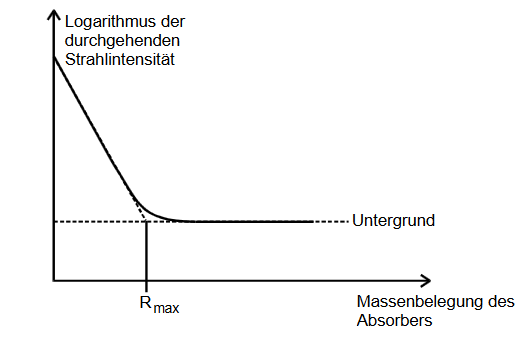
\includegraphics[width=0.6\textwidth]{abf.PNG}
  \caption{Darstellung der Absorptionskurve.\cite{sample}}
  \label{fig:abf}
\end{figure}
Die maximale Reichweite $R_\mathrm{max}$ wird von den energiereichsten Elektronen bestimmt, über diese kann
auf die freiwerdende Gesamtenergie über folgende Beziehung:
\begin{align}
E_\mathrm{max}=1,92\sqrt{R^2_\mathrm{max}+0,22R_\mathrm{max}}\label{eqn:emax}
\end{align}
geschlossen werden.
